\documentclass[12pt]{article}

\usepackage[a4paper,top=0.4in,bottom=0.4in,left=0.75in,right=0.75in]{geometry}
\usepackage{array}
\usepackage{graphicx}
\usepackage{enumitem}

\setlength{\parindent}{0pt}
\setlength{\parskip}{0.55em}
\renewcommand{\arraystretch}{1.15}

% Section labels in all caps.
\newcommand{\reportlabel}[1]{\vspace{0.6em}\textbf{\MakeUppercase{#1}}\par\vspace{0.3em}}

% Header image
\newcommand{\headerimageplaceholder}{%
    \noindent
\includegraphics[width=\textwidth]{images/rvce_logo_header}\par
    \vspace{0.8em}
}

\begin{document}
\pagestyle{empty}

\headerimageplaceholder

\begin{tabular}{|p{0.28\textwidth}|p{0.67\textwidth}|}
\hline
\textbf{Team ID} & 3 \\\hline
\textbf{Semester} & 7\textsuperscript{th} \\\hline
\textbf{Team Details} &
\begin{tabular}{|p{0.05\linewidth}|p{0.22\linewidth}|p{0.22\linewidth}|p{0.375\linewidth}|}
\hline
\textbf{} & \textbf{Program} & \textbf{USN} & \textbf{Name} \\\hline
1. & B.E. (CSE) & 1RV23CS291 & Vishal K Bhat \\\hline
2. & B.E. (CSE) & 1RV23CS265 & Tallam Sri Sai Subramanyam \\\hline
3. & B.E. (CSE) & 1RV23CS307 & Medha Sanketh \\\hline
4. & B.E. (ISE) & 1RV23IS145 & Avinash Anish \\\hline
\end{tabular} \\\hline
\textbf{Project Title} & Natural Language Search Engine for Large-Scale Video Repositories \\\hline
\textbf{Centre of Excellence} & Centre of Excellence in Computer Vision Research \\\hline
\multicolumn{2}{|c|}{\textbf{Internal Guide}} \\\hline
\textbf{Name \newline Designation \& Department} & Dr. Pratiba D \newline Associate Professor, Department of CSE \\\hline
\end{tabular}

\reportlabel{Introduction:}
Large video repositories such as surveillance archives, lecture libraries and media collections are indexed by nothing but filename and clock time, so footage can be retrieved only by when it was recorded, while what a user actually possesses is a \textbf{description} of the event. This project builds a \textbf{natural language search engine over video}: vision-language, speech and retrieval models derive a searchable description of footage that carries none, forming a \textbf{Retrieval-Augmented Generation (RAG) pipeline over video} that returns timestamped, playable moments and cited answers rather than a list of files.

\reportlabel{Objectives:}

\begin{enumerate}[noitemsep, topsep=0pt, leftmargin=1.5em]
    \item To develop a pipeline that renders a recording searchable by description, without relying on shot boundaries, speech or visual salience.
    \item To build a multi-vector semantic index returning ranked moments with \texttt{mm:ss} timecodes under typed filters.
    \item To derive video-level understanding (summary, chapters, events, entities and anomalies) and answer questions against it with mandatory citations.
    \item To deliver a multi-tenant web workspace with an LLM agent front end, over a self-describing HTTP API, and benchmark retrieval quality and latency at repository scale.
\end{enumerate}

\reportlabel{Methodology:}

\begin{enumerate}[noitemsep, topsep=0pt, leftmargin=1.5em]
    \item \textbf{Chunking:} Four fused boundary detectors: speaker change (pyannote), silence (Silero VAD), hard cuts (PySceneDetect) and semantic drift (OpenCLIP). A signal that produces no events cedes its weight to those that did
    \item \textbf{Analysis:} Scene, person, object (YOLO11), on-screen text (EasyOCR) and speech (faster-whisper) analyzers, with the vision-language model gated by the cheap detectors and adaptive frame sampling
    \item \textbf{Indexing:} Local BGE embeddings into Qdrant, five named vectors per chunk with a typed payload for structured filtering
    \item \textbf{Aggregation \& QA:} Twelve dependency-ordered aggregators; questions routed to the aggregate able to answer them, answers synthesised with cited moments
    \item \textbf{Application:} FastAPI service and Next.js workspace with an agent tool loop; Supabase Postgres, Auth and Storage with row-level tenancy
\end{enumerate}

\reportlabel{Software Requirements:}

\small
\begin{tabular}{|p{0.22\textwidth}|p{0.22\textwidth}|p{0.22\textwidth}|p{0.22\textwidth}|}
\hline
Python 3.13 & FastAPI / Uvicorn & PyTorch (CUDA) & Transformers \\\hline
Qdrant (vector DB) & sentence-transformers & faster-whisper & YOLO11 / EasyOCR \\\hline
pyannote.audio & Silero VAD / PySceneDetect & OpenCLIP / OpenCV & Next.js / React / TypeScript \\\hline
Supabase (Postgres, Auth, Storage) & Vercel AI SDK & Docker & Git \\\hline
\end{tabular}
\normalsize

\reportlabel{Hardware Requirements:}

\small
\begin{tabular}{|p{0.22\textwidth}|p{0.22\textwidth}|p{0.22\textwidth}|p{0.22\textwidth}|}
\hline
\textbf{Component} & \textbf{Specification} & \textbf{Component} & \textbf{Specification} \\\hline
Processor & Intel i5/i7 or equiv. & RAM & 16\,GB recommended \\\hline
GPU & NVIDIA CUDA, 8\,GB VRAM & Storage & 50\,GB (media cache + weights) \\\hline
\end{tabular}
\normalsize

\reportlabel{Concept Mockup:}

\begin{center}
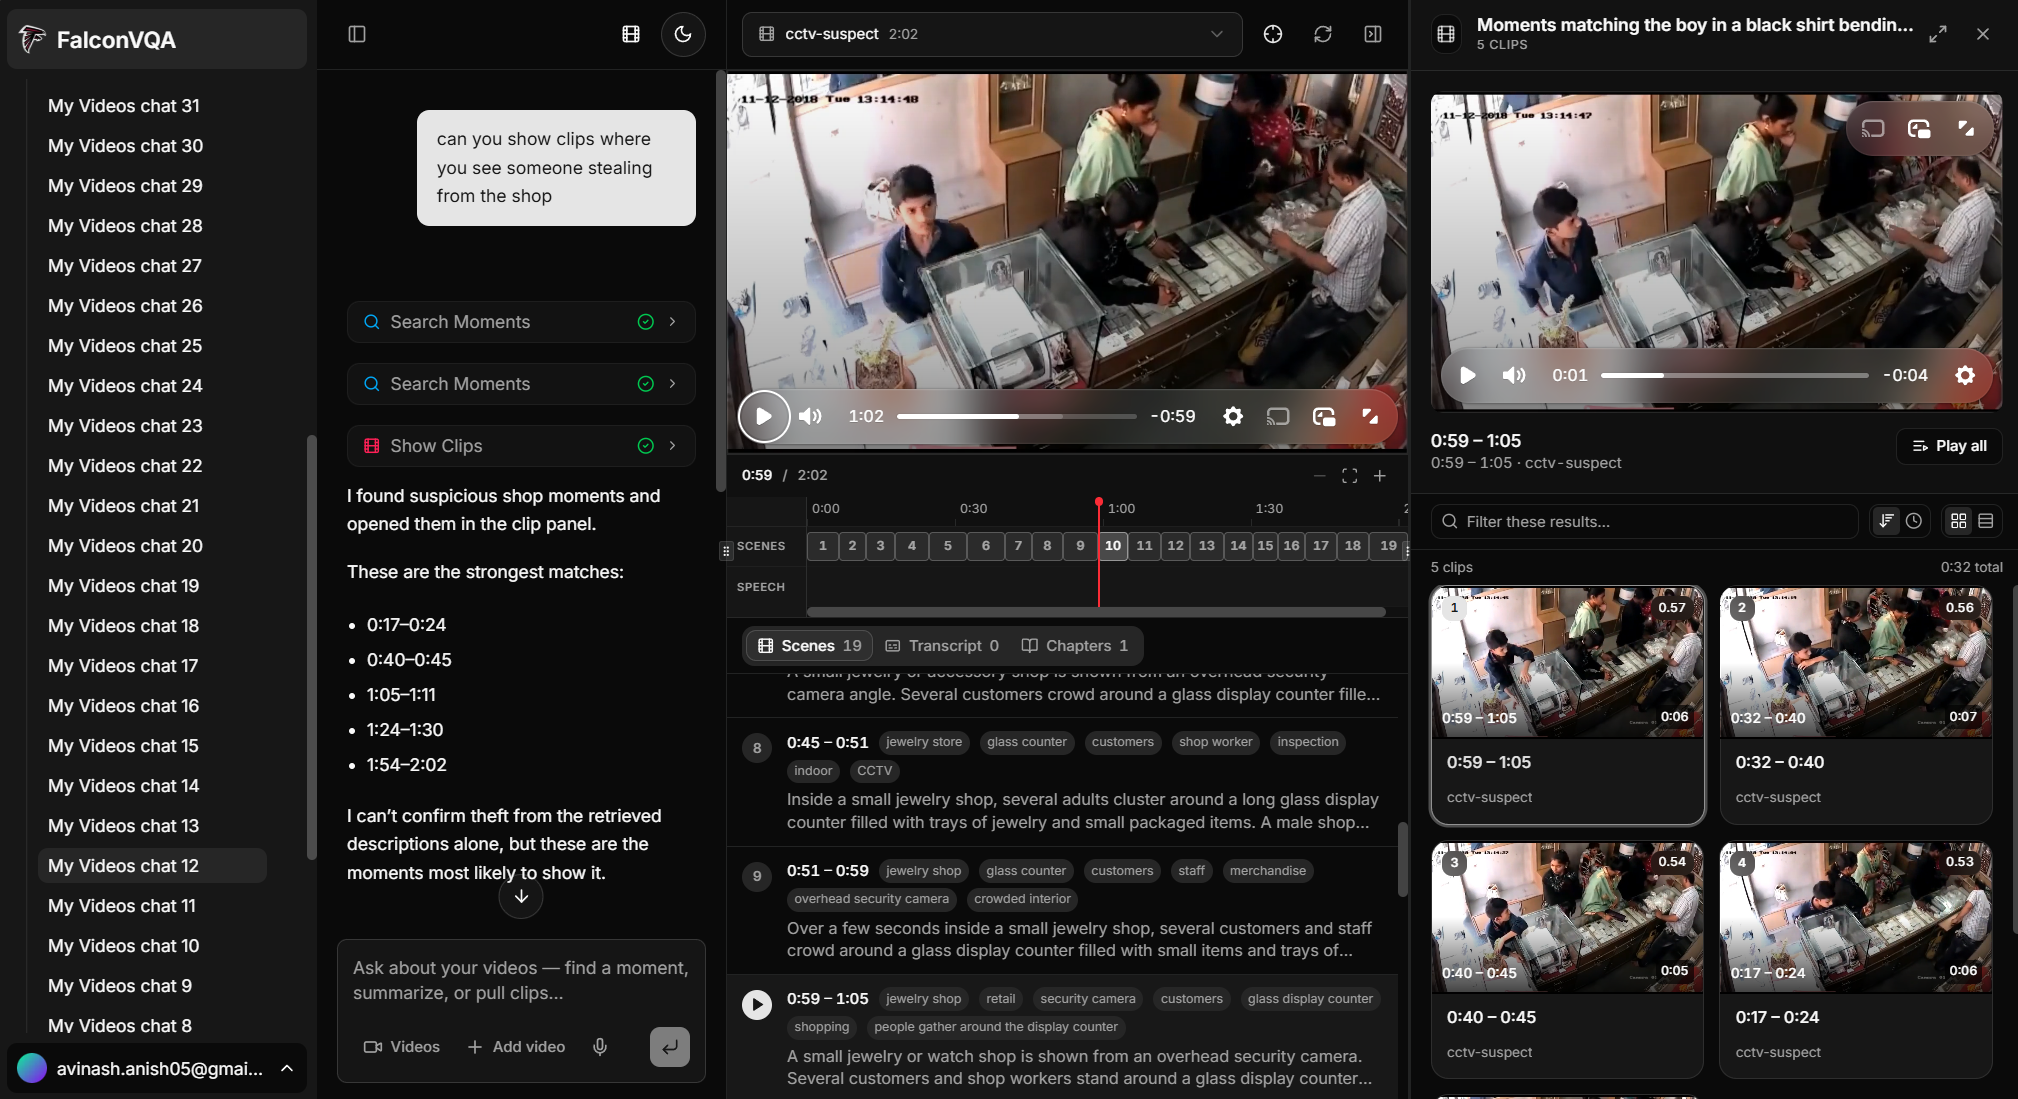
\includegraphics[width=0.95\textwidth]{images/falconvqa-agent}\par
\vspace{0.4em}
{\small Concept mockup of the proposed workspace: a plain-language request resolved into
ranked moments, with the retrieved clips and their \texttt{m:ss} timecodes shown alongside
the answer.}
\end{center}

\end{document}
